\section{Motivation and Observation}
\label{sec:observation}

\begin{figure}
	\centering
	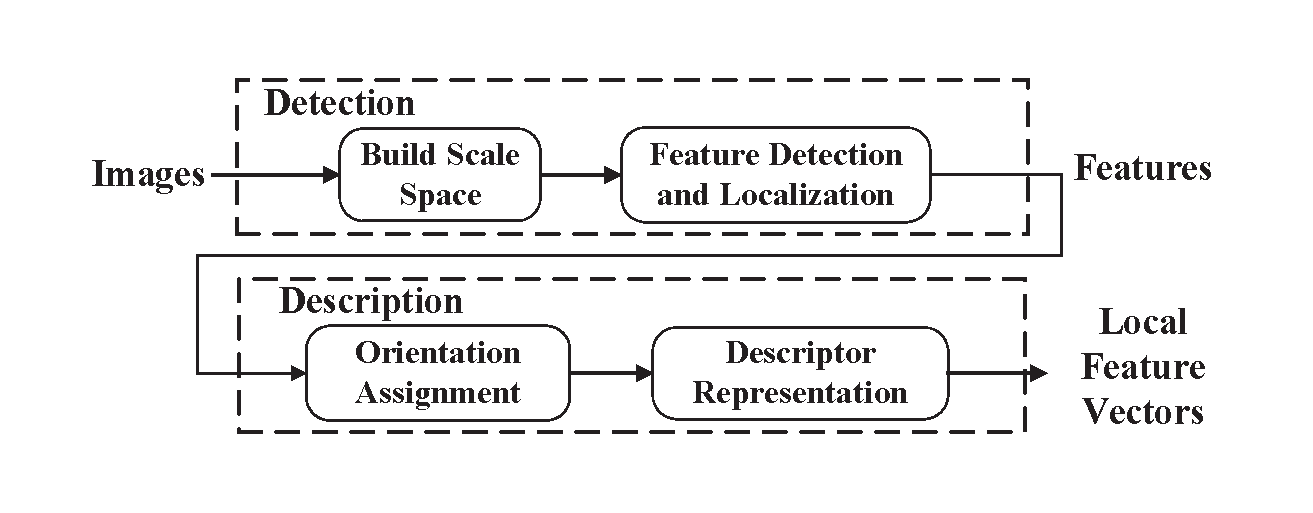
\includegraphics[width=3.0in]{images/fig-workflow.eps}
	\caption{Process flow of a typical local feature descriptor.}
	\label{fig:workflow}
\end{figure}

\subsection{Motivation}

A local feature descriptor detects local features which are invariant to image scaling and rotation. Some of them are even invariant to changes in illumination and 3D camera viewpoint. Typically, it consists of detection stage and description stage. The detailed process flow is shown in Figure~\ref{fig:workflow}. In the detection stage, scale invariant features are detected. Then, in the description stage, each point is assigned one or more orientations based on local image gradient directions, which is the key step in achieving invariance to rotation. At the end of the description stage, each detected feature should be computed to a high dimension vector.

There exist two major problems for local feature descriptors. First, computing high dimension feature vectors is relatively slow. Second, many of the detected local features are useless or unimportant. Salient region~\cite{huang2009image,liang2010salient} can be used here to solve the two problems by removing local features outside important area. Since detecting salient regions is also a somehow time-consuming computation, when used together with local feature descriptor, the final computation performance can not be improved as expected.

To overcome these performance issues, we choose to involve a approximate approach for salient region detection. And this approach is based on the following observations.

\subsection{Observation}

As shown in Figure~\ref{fig:observations}, feature points can be represented as points, where the radius of each point equals its scale. After studying carefully on the distribution of feature points, we get three major observations:

\begin{description}
	
	\item[Observation 1] \desclabel{itm:observation_1} \textit{Local features in the salient region are close to each other, while noises and unimportant features are far away from them.} As shown in Figure \ref{fig:observation_1}, local features in the salient region (green box) gather together and many obvious unimportant local features locate far away from that box. 

	\item[Observation 2] \desclabel{itm:observation_2} \textit{The region with most local features is the preferred salient region.} Also from Figure \ref{fig:observation_1}, the preferred green box has much more local features than other two yellow boxes. 

	\item[Observation 3] \desclabel{itm:observation_3} \textit{There may exist several salient regions in one image, which are observed as clusters of local features.} For example, the photo in Figure \ref{fig:observation_2} contains two objects, a person and a stop sign, which shape two salient regions following the clusters of local features.

\end{description}

Observation~\ref{itm:observation_1} and \ref{itm:observation_2} indicate a possibility that we can compute the salient region directly from the distribution of local features. In addition, Observation~\ref{itm:observation_3} means it's necessary to deal with multiple salient regions if there exist clusters of local features.
